This chapter discusses tests the hypothesis stated in the Methodology chapter. To arrive at the hypothesis tests, this chapter will first discuss the descriptives of the dataset. Thereafter the research sub questions are investigated.
\section{Descriptive statistics}
Descriptive statistics are used to inform the reader about the general characteristics of the dataset used to test the hypothesis. Preferably these characteristics resemble the characteristic of the wider population to allow for generalized statements. Therefore, the firms from dataset analyzed were compared to the JSE All Share Index. The JSE All Share Index is the broad based Index of the Johannesburg Stock Exchange. The table below compares the sector weighting for the B-BBEE sample and the JSE All Share Index (equal weighted) as of latest date. The equal weight of latest date for the JSE All Share Index was retrieved from Thomson Reuters Datastream. This index was chosen because only the latest date (as of 30th April 2019) and names (no weight) were available for the constituents of the JSE All Share Index.
\begin{table}[H] %H forces the position of the table at the line where you place it (not on a separate page etc) -https://tex.stackexchange.com/questions/121155/how-to-adjust-a-table-to-fit-on-page https://tex.stackexchange.com/questions/332528/increasing-the-space-between-two-rows?rq=1
\centering
\caption{Relative bias sample versus JSE All Share Index 2019} 
\resizebox{\textwidth}{!}{\begin{tabular}{ccccccccc}

  \bottomrule
  \\
 Year & Basic Materials & Consumer Goods & Consumer Services & Financials   & Healthcare   & Industrials & Technology   & Telecommunications \\ \\
  \midrule
2004 & 6\%             & 0\%            & 5\%               & -18\%      & -3\%       & 4\%         & 4\%        & 1\%                \\
2005 & 2\%             & 2\%            & -2\%              & -14\%      & -1\%       & 4\%         & 8\%        & 1\%                \\
2006 & 2\%             & 4\%            & 1\%               & -18\%      & -1\%       & 1\%         & 9\%        & 1\%                \\
2007 & 4\%             & -3\%           & 1\%               & -9\%       & -1\%       & -2\%        & 9\%        & 1\%                \\
2008 & -3\%            & -5\%           & -5\%              & -11\%      & -1\%       & 9\%         & 13\%       & 3\%                \\
2009 & -8\%            & -1\%           & 1\%               & -11\%      & 1\%        & 11\%        & 9\%        & -2\%               \\
2010 & -8\%            & -3\%           & -2\%              & -14\%      & 1\%        & 14\%        & 9\%        & 3\%                \\
2011 & -6\%            & -3\%           & -5\%              & -13\%      & 1\%        & 16\%        & 8\%        & 3\%                \\
2012 & -4\%            & -5\%           & -4\%              & -13\%      & -1\%       & 16\%        & 9\%        & 1\%                \\
2013 & -6\%            & -3\%           & -4\%              & -11\%      & 1\%        & 11\%        & 8\%        & 4\%                \\
2014 & -8\%            & -1\%           & -5\%              & -13\%      & 1\%        & 14\%        & 8\%        & 4\%                \\
2015 & -9\%            & -3\%           & -4\%              & -8\%       & 1\%        & 16\%        & 8\%        & -1\%               \\
2016 & -3\%            & -5\%           & -10\%             & -9\%       & -4\%       & 23\%        & 8\%        & 1\%                \\
2017 & -3\%            & -6\%           & 13\%              & -31\%      & 2\%        & 26\%        & -1\%       & -1\%               \\
2018 & -3\%            & -5\%           & -4\%              & -14\%      & -1\%       & 19\%        & 8\%        & -1\%  \\ 
   \bottomrule
\end{tabular}}
\end{table} 

This table shows the percentage of observations in any of the respective sectors for the JSE All Share equal weight, and the firms for which B-BBEE rank was available. Recall that the JSE All Share equal weight was retrieved from one point in time, therefore the percentage of observations in any of the sectors of the JSE All Share equal weight was static through time. The constituents, and therefore the weight of each sector for dataset used for analysis however did change annually. In the dataset used for analysis there was a significant bias towards Industrials, compared to the JSE All Share equal weight. This might be due to the nature of this sector. This sector has a larger incentive  to comply to B-BBEE, which causes firms in the Industrial sector to place extraordinary effort into achieving high B-BBEE aggregate scores, eventually causing the Empowerdex top 100 list to consists of more Industrial firms. Most firms in the Industrial sector were active in the construction business. Recall from the segment Compliance effects in the Theory chapter, that firms that reach B-BBEE targets and beyond receive higher B-BBEE aggregate score which is a consideration into tendering for government contracts. Further, under the preferential procurement (a B-BBEE element) any firm supplying goods or services to the government or other public entities must ensure that the supplies purchased are from B-BBEE compliant firms [7, p546; 3,5 p9]. Put straightforward, a firm operating in the construction sector will probably have either a direct or indirect relationship with the government which incentives this firm to reach a high B-BBEE score. This most likely explains the overrepresentation of firms from the Industrial sector in this dataset for analysis. It is interesting to note the increase in bias toward the Industrial sector in this dataset compared to the JSE All Share equal weight after each amendment to the Codes of good practise. These amendments occured in 2007 and in 2013 as mentioned in the section “The mechanics of the B-BBEE scorecard”. Prior to 2007 the overrepresentation was about 4\%, between 2007 and 2013 about 15\%, and after 2013 24\%. Contrary, the dataset for analysis underrepresented the Financials sector. This could be explained from a similar philosophy, that the representation bias in the dataset for analysis has been fueled by the incentive of a firm to comply to BBBEE. Financials, such as banks could have a lesser incentive to achieve a high B-BBEE score as these firms are not directly tendering on government contracts, nor are these firms active as suppliers. However, from the perspective of signalling effects it is surprising that Financials are underrepresented. Recall from the section B-BBEE and signalling effects that consumer behavior could express their values regarding empowerment in their consumption pattern [34, p378]. This could mean that consumers would demand B-BBEE compliance from their banks. In the section The first phase of BEE, BEE as the transfer of shares it was noted that a Financials, Sanlam was the first South African firm to implement a form of BEE by transferring 10\% of ownership to Black people. Therefore the underrepresentation is surprising and inviting for further research.

Despite these difference, the top 3 dominant sectors of the JSE All Share equal weight; Basic Materials, Consumer Service and Financials are also dominant in the B-BBEE rank observations. The smaller sectors; Technology, Health Care and Telecommunication displayed at most overseeable deviations between the B-BBEE rank observations and JSE All Share Index. The JSE All Share Index consisted of 164 firms, of which 125 were included in the B-BBEE rank observations at some point in time. Therefore, the dataset used for analysis was representative of the Johannesburg Stock Exchange listed firms.

The maximum amount of observations, given 60 firms for 15 years equals 900. Below an overview of the variables for Model 1, the FF (Fama and French based) model.  
\begin{table}[H] %H forces the position of the table at the line where you place it (not on a separate page etc) -https://tex.stackexchange.com/questions/121155/how-to-adjust-a-table-to-fit-on-page https://tex.stackexchange.com/questions/332528/increasing-the-space-between-two-rows?rq=1
\centering
\caption{Descriptive statistics variables} 
\resizebox{\textwidth}{!}{\begin{tabular}{ccccccccc}

  \bottomrule
  \\
 & BP    & SIZE  & EP  & BPIndex\_YR1 & SIZEIndex\_YR1 & MarketPremium\_YR1 & RiskFreeReturn\_YR1 & PriceLogReturn\_YR1 \\ \\
  \midrule
count & 816   & 900     & 835      & 15           & 15             & 15                 & 15                  & 900                 \\
mean  & 0.90  & 36024   & -11.50   & 6\%          & 2\%            & 9\%                & 8\%                 & 14\%                \\
std   & 2.42  & 96943   & 221.03   & 6\%          & 7\%            & 23\%               & 1\%                 & 47\%                \\
min   & -0.47 & 3       & -4670.81 & 0\%          & -15\%          & -20\%              & 7\%                 & -95\%               \\
25\%  & 0.34  & 1522    & 5.10     & 3\%          & -1\%           & -5\%               & 8\%                 & -12\%               \\
50\%  & 0.55  & 7653    & 7.70     & 6\%          & 4\%            & 3\%                & 9\%                 & 10\%                \\
75\%  & 0.88  & 26091   & 10.30    & 8\%          & 8\%            & 18\%               & 9\%                 & 31\%                \\
max   & 55.66 & 1434027 & 65.39    & 23\%         & 12\%           & 67\%               & 10\%                & 756\%     \\ 
   \bottomrule
\end{tabular}}
\end{table} 
The average Price log return varied widely. The standard deviation was 47.6\%, and the difference between the minimum and maximum observation price log return for one year equaled more than 800\%. Similarly the book to market ratio and size variable varied greatly. The minimum BP was negative, indicating a firm with negative book value. This indicates negative equity value, or a company in severe distress. The number of observations on the book to market ratio equaled 816, indicating that of 900 observations there was no book to market ratio available for 84 observations. The SIZE variable indicates that both very small firms and very large firms were available in the dataset used for analysis. The indices, BP, SIZE, MarketPremium, and RiskFreeReturn only showed 1 value for each year, hence 15 observations were yielded for these variables. Recall that the RiskFreeReturn equals 10 years South African government bond. The RiskFreeReturn remained, compared to the other variables,  relatively immune from variability. The bottom 25 percentile  observation equaled 8.1\% and the top 75 percentile observation equaled 8.7\%.

To prevent impact from outliers, the dataset was supplemented with a dataset adjusted for outliers. The descriptives for this dataset can be viewed below.
\begin{table}[H] 
\centering
\caption{Descriptive statistics variables outlier adjusted} 
\resizebox{\textwidth}{!}{\begin{tabular}{ccccccccc}
  \bottomrule
  \\
 & BP    & SIZE   & EP      & BPIndex\_YR1 & SIZEIndex\_YR1 & MarketPremium\_YR1 & RiskFreeReturn\_YR1 & PriceLogReturn\_YR1 \\ \\
  \midrule
count & 816   & 900    & 835      & 15           & 15             & 14                 & 14                  & 900                 \\
mean  & 0.77  & 29618  & -11.50   & 4\%          & 4\%            & 4\%                & 17\%                & 14\%                \\
std   & 0.79  & 52727  & 221.03   & 3\%          & 4\%            & 21\%               & 1\%                 & 40\%                \\
min   & -0.47 & 3      & -4670.81 & 0\%          & -3\%           & -27\%              & 15\%                & -95\%               \\
25\%  & 0.34  & 1522   & 5.10     & 2\%          & 1\%            & -7\%               & 17\%                & -12\%               \\
50\%  & 0.55  & 7653   & 7.70     & 4\%          & 3\%            & 1\%                & 18\%                & 10\%                \\
75\%  & 0.88  & 26091  & 10.30    & 6\%          & 6\%            & 7\%                & 18\%                & 31\%                \\
max   & 4.84  & 225857 & 65.39    & 11\%         & 12\%           & 50\%               & 19\%                & 189\%      \\
   \bottomrule
\end{tabular}}
\end{table} 
This dataset for constrained the minimum value for the book to market ratio, size and PriceLogReturn to -2 times standard deviation from the mean, and the maximum value to +2 times standard deviation from the mean. Because PriceLogReturn was adjusted the Indices BP, SIZE and MarketPremium, which are based upon PriceLogReturn, also changed. The outlier adjusted dataset, still displayed variability, however at a much lower rate as can be viewed from the significantly lower maximum value for BP, SIZE and PriceLogReturn. It is interesting to note that the variability of the MarketPremium rose as result of the outlier adjustment for the PriceLogReturn. This indicates that as outliers were excluded from PriceLogReturn, correlations increased between firms PriceLogReturn and therefore the variability of the MarketPremium increased.

The correlation matrix suggests that multicollinearity did not exist in the dataset used for analysis. Below the correlation matrix for the dataset, not adjusted for outliers. 
\begin{table}[H] 
\centering
\caption{Correlation matrix} 
\resizebox{\textwidth}{!}{\begin{tabular}{rrrrrrrrrr}
  \bottomrule
     & 1     & 2     & 3     & 4     & 5     & 6     & 7     & 8     & 9 \\
  \midrule
BP (1)                  & 1.00  & -0.08 & -0.02 & 0.01  & -0.04 & -0.07 & 0.04  & 0.04  & -0.05 \\
SIZE (2)                & -0.08 & 1.00  & 0.03  & -0.03 & -0.05 & 0.06  & -0.04 & -0.06 & 0.04  \\
E2P (3)                 & -0.02 & 0.03  & 1.00  & 0.03  & -0.02 & 0.01  & 0.05  & 0.00  & 0.08  \\
BPIndex\_YR1 (4)        & 0.01  & -0.03 & 0.03  & 1.00  & 0.00  & -0.11 & -0.34 & 0.06  & -0.20 \\
BBBEE\_Rank (5)         & -0.04 & -0.05 & -0.02 & 0.00  & 1.00  & 0.00  & 0.00  & 0.00  & -0.03 \\
SIZEIndex\_YR1 (6)      & -0.07 & 0.06  & 0.01  & -0.11 & 0.00  & 1.00  & -0.60 & -0.28 & -0.15 \\
MarketPremium\_YR1 (7)  & 0.04  & -0.04 & 0.05  & -0.34 & 0.00  & -0.60 & 1.00  & -0.07 & 0.39  \\
RiskFreeReturn\_YR1 (8) & 0.04  & -0.06 & 0.00  & 0.06  & 0.00  & -0.28 & -0.07 & 1.00  & -0.05 \\
PriceLogReturn\_YR1 (9) & -0.05 & 0.04  & 0.08  & -0.20 & -0.03 & -0.15 & 0.39  & -0.05 & 1.00                 \\ 
   \bottomrule
\end{tabular}}
\end{table} 

An overview of the correlations on two, three, four and five years basis can be found in Appendix A. The correlation matrix for the outlier adjusted dataset shows as similar picture, as can be viewed below.
\begin{table}[H] 
\centering
\caption{Correlation matrix} 
\resizebox{\textwidth}{!}{\begin{tabular}{rrrrrrrrrr}
  \bottomrule
     & 1     & 2     & 3     & 4     & 5     & 6     & 7     & 8     & 9 \\
  \midrule
BP (1)                  & 1.00  & -0.23 & -0.08 & 0.02  & -0.02 & 0.03  & -0.10 & 0.06  & -0.17 \\
SIZE (2)                & -0.23 & 1.00  & 0.04  & 0.00  & -0.03 & 0.04  & -0.01 & -0.08 & 0.06  \\
E2P (3)                 & -0.08 & 0.04  & 1.00  & 0.05  & -0.02 & 0.04  & 0.05  & 0.00  & 0.09  \\
BPIndex\_YR1 (4)        & 0.02  & 0.00  & 0.05  & 1.00  & 0.00  & 0.53  & -0.34 & -0.12 & -0.16 \\
BBBEE\_Rank (5)         & -0.02 & -0.03 & -0.02 & 0.00  & 1.00  & 0.00  & 0.00  & 0.00  & -0.01 \\
SIZEIndex\_YR1 (6)      & 0.03  & 0.04  & 0.04  & 0.53  & 0.00  & 1.00  & -0.65 & -0.29 & -0.24 \\
MarketPremium\_YR1 (7)  & -0.10 & -0.01 & 0.05  & -0.34 & 0.00  & -0.65 & 1.00  & -0.27 & 0.46  \\
RiskFreeReturn\_YR1 (8) & 0.06  & -0.08 & 0.00  & -0.12 & 0.00  & -0.29 & -0.27 & 1.00  & -0.05 \\
PriceLogReturn\_YR1 (9) & -0.17 & 0.06  & 0.09  & -0.16 & -0.01 & -0.24 & 0.46  & -0.05 & 1.00                \\ 
   \bottomrule
\end{tabular}}
\end{table} 

The outlier adjusted correlation matrix shows more pronounced correlations. For example the correlation between BP and SIZE is -0.23 in the outlier adjusted dataset versus -0.08 in the original dataset. Nonetheless, the correlation between these variables is low to negative. It can also be observed from this outlier adjusted correlation matrix that the market, contrary intuition based on the Fama French theory, indicates a negative correlation between BP and PriceLogReturn. Recall from section “Previous research on the relationship between B-BBEE scores and firm performance” that Fama and French state that the market undervalues distressed, high book to market ratio firms, and therefore these firms tend to outperform low book to market ratio firms [52, p1975]. This relationship is elusive in the context of this dataset. On the other hand the correlation between MarketPremium and PriceLogReturn did display a higher correlation, 0.46. Therefore, the dataset suggests that PriceLogReturn for a firm was mostly determined by movement of the general market. This, in the context of a developing/emerging market such as South Africa, seems perfectly logical as these markets are not as mature as the United States, Japanese or European markets upon which the Fama French study were based. Nonetheless the unexpected correlation between BP and PriceLogReturn does raise concerns on the appropriateness of BP as a control variable in this study.
\section{Regression results}
The dataset was tested on both subsections of the dataset (i.e. particular years) and the entire dataset. First is discussion on the result of analysis on the entire dataset. 
\subsection{Relationship between B-BBEE policy and firm performance 2004 -2018}
This section concerns the research sub question: “What was the long term relationship between  Broad-Based Black Economic Empowerment policy on firm profitability of the Johannesburg Stock Exchange-listed companies over the period 2004 - 2018?”. The regression results of the original dataset, not adjusted for outliers, for Model 1, the FF model looks as follows:
\begin{table}[H] 
\tiny %https://tex.stackexchange.com/questions/27097/changing-the-font-size-in-a-table
\centering
\caption{Regression Model 1, 2004 - 2018} 
\resizebox{\textwidth}{!}{\begin{tabular}{lrrrrr}
  \bottomrule
     &     1     &     2     &     3      &     4     &     5      \\
  \midrule
BP                 & -0.2480   & -0.4555   & -1.1840    & 0.3650    & 1.2904     \\
                   & (0.3197)  & (0.8511)  & (1.5824)   & (2.5089)  & (2.1644)   \\
BBBEE_Rank         & -0.0006   & -0.0028*  & -0.0069*** & -0.0065*  & -0.0017    \\
                   & (0.0009)  & (0.0016)  & (0.0026)   & (0.0034)  & (0.0046)   \\
SIZE               & 0.8076**  & 0.5197    & 0.6443     & 0.6603    & -0.1533    \\
                   & (0.3248)  & (0.5360)  & (0.7693)   & (1.1358)  & (1.1300)   \\
MarketPremium      & 0.9686*** & 1.0702*** & 1.1230***  & 1.4520*** & 1.6534***  \\
                   & (0.1079)  & (0.1748)  & (0.3680)   & (0.5178)  & (0.3945)   \\
RiskFreeReturn     & 0.6521    & -0.1951   & 0.8228     & -2.7341   & -4.1080    \\
                   & (2.2691)  & (2.9432)  & (3.6206)   & (7.5388)  & (7.9526)   \\
Consumer Goods     & 0.0369    & 0.2265    & 0.1400     & 1.7100    & 2.9063     \\
                   & (0.2143)  & (0.5548)  & (1.0675)   & (2.9893)  & (4.0711)   \\
Financials         & 0.0558    & 0.3282    & 0.3099     & 1.8070    & 2.9933     \\
                   & (0.2090)  & (0.5489)  & (1.0607)   & (2.9764)  & (4.0449)   \\
Technology         & -0.0488   & 0.2580    & 0.2805     & 1.8074    & 3.0038     \\
                   & (0.2127)  & (0.5551)  & (1.0666)   & (2.9762)  & (4.0513)   \\
Healthcare         & 0.0960    & 0.5821    & 0.5522     & 2.1466    & 3.4400     \\
                   & (0.2165)  & (0.5585)  & (1.0739)   & (2.9911)  & (4.0623)   \\
Industrials        & -0.0384   & 0.1635    & 0.0480     & 1.4233    & 2.2926     \\
                   & (0.2061)  & (0.5464)  & (1.0565)   & (2.9752)  & (4.0371)   \\
Consumer Services  & 0.0634    & 0.2392    & 0.1807     & 1.6321    & 2.7102     \\
                   & (0.2102)  & (0.5533)  & (1.0664)   & (2.9819)  & (4.0610)   \\
Basic Materials    & 0.0184    & 0.1657    & 0.0090     & 1.5287    & 2.4668     \\
                   & (0.2115)  & (0.5537)  & (1.0651)   & (2.9778)  & (4.0566)   \\
Telecommunications & 0.0742    & 0.2379    & 0.1742     & 1.5765    & 2.4642     \\
                   & (0.2201)  & (0.5583)  & (1.0682)   & (2.9831)  & (4.0483)   \\
N                  & 816       & 752       & 694        & 638       & 582        \\
R^2                 & 0.18      & 0.22      & 0.26       & 0.14      & 0.10       \\
   \bottomrule
Standard errors in parentheses.
* p<10\%, ** p<5\%, ***p<1\%
\end{tabular}}
\end{table} 

There are 5 columns visible in this table, these tables represent the share price returns time horizon. Therefore column 1 represent the 1 year share price return, column 2 represents the two year forward share price return, etc. From this model, under the specifications stated (no adjustment for outliers), r squared for all time horizons exceed 0.10. Merwe and Ferreira, in their study, note that a r squared of 5.6\% is acceptable to investigate the relationship between B-BBEE score and share price return. Therefore, the model results of more than 0.10, can be interpreted as sufficient to capture the relationship between B-BBEE rank and share price return. This model finds a negative relationship between B-BBEE rank and share price return, significant on a two, three and four years time horizon. It has to be noted that the magnitude, especially compared to the coefficients of other independent variable is small. In comparison, the magnitude of the market premium is far larger, and significant over the five time horizons. This suggests that the impact of B-BBEE is relatively small, but negative. Merwe and Ferreira also observed a same small negative relationship between B-BBEE and share price return [7, p552]. Using the different time horizon, this model shows that the negative coefficient of B-BBEE rank increases up until the 4 years time horizon, from -0.0006 to -0.065. Mehta and Ward suggested that the market has an initial response to a B-BBEE rank, which is more positive, and as the market processes information, the response to the B-BBEE rank becomes more pronounced [27, p89]. This initial more positive response could indicate the positive signalling effect. Over the time the costs of B-BBEE outweigh the benefits. Thus, this FF model without outlier adjustment favors the acceptance of alternative hypothesis. The long term relationship between B-BBEE aggregate score and share price return of Johannesburg Stock Exchange-listed companies is not positive. The null hypothesis is rejected.

To check for robustness, this study removed outliers from the dataset. Adjusting for outliers shows the following results:
\begin{table}[H] 
\tiny %https://tex.stackexchange.com/questions/27097/changing-the-font-size-in-a-table
\centering
\caption{Regression Model 1 - outlier adjusted, 2004 - 2018} 
\resizebox{\textwidth}{!}{\begin{tabular}{lrrrrr}
  \bottomrule
     &     1     &     2     &     3      &     4     &     5      \\
  \midrule
BP                 & -0.4858   & -1.8037   & -2.0434   & -2.5375*  & -1.0682   \\
                   & (0.4961)  & (1.2019)  & (1.5805)  & (1.4165)  & (1.7208)  \\
BBBEE_Rank         & 0.0002    & -0.0023*  & -0.0040** & -0.0046** & -0.0031   \\
                   & (0.0008)  & (0.0012)  & (0.0018)  & (0.0023)  & (0.0031)  \\
SIZE               & 1.4892*** & 1.4440*** & 1.9992*** & 1.5684*   & 0.7834    \\
                   & (0.5035)  & (0.4597)  & (0.5777)  & (0.8307)  & (1.2044)  \\
MarketPremium      & 0.9909*** & 0.7264*** & 0.5739    & 0.6428    & 0.9448**  \\
                   & (0.0889)  & (0.2324)  & (0.4437)  & (0.3912)  & (0.3946)  \\
RiskFreeReturn     & -0.9639   & -5.2936** & -6.9621** & -3.7378   & -4.6235   \\
                   & (2.3277)  & (2.4482)  & (3.0451)  & (2.5987)  & (3.0165)  \\
Consumer Goods     & 0.1620    & 1.1208*** & 2.2522*** & 2.0092**  & 3.1361**  \\
                   & (0.2098)  & (0.4083)  & (0.7774)  & (0.9581)  & (1.4945)  \\
Financials         & 0.1339    & 1.1070*** & 2.1980*** & 1.9381**  & 3.0821**  \\
                   & (0.2058)  & (0.4012)  & (0.7659)  & (0.9435)  & (1.4760)  \\
Technology         & 0.0557    & 1.0409**  & 2.0749*** & 1.5954*   & 2.5532*   \\
                   & (0.2091)  & (0.4069)  & (0.7730)  & (0.9501)  & (1.4821)  \\
Healthcare         & 0.2218    & 1.3349*** & 2.5125*** & 2.3881**  & 3.7449**  \\
                   & (0.2115)  & (0.4115)  & (0.7734)  & (0.9552)  & (1.4895)  \\
Industrials        & 0.0540    & 0.9886**  & 1.9611**  & 1.5478*   & 2.4982*   \\
                   & (0.2035)  & (0.3977)  & (0.7609)  & (0.9391)  & (1.4675)  \\
Consumer Services  & 0.1520    & 1.1381*** & 2.2232*** & 1.8841**  & 2.9608**  \\
                   & (0.2070)  & (0.4056)  & (0.7723)  & (0.9489)  & (1.4848)  \\
Basic Materials    & 0.1664    & 1.0613*** & 2.1641*** & 1.7577*   & 2.7730*   \\
                   & (0.2072)  & (0.4061)  & (0.7780)  & (0.9528)  & (1.4871)  \\
Telecommunications & 0.1557    & 1.1154*** & 2.2015*** & 1.7467*   & 2.6537*   \\
                   & (0.2129)  & (0.4132)  & (0.7783)  & (0.9564)  & (1.4832)  \\
N                  & 757       & 693       & 635       & 579       & 523       \\
R^2                 & 0.24      & 0.20      & 0.14      & 0.15      & 0.14      \\
   \bottomrule
Standard errors in parentheses.
* p<10\%, ** p<5\%, ***p<1\%
\end{tabular}}
\end{table} 

Here, the relationship between B-BBEE rank and share price return on a one-year time horizon is slightly positive albeit not significant. On the two, three and four years time horizon, the relationship between B-BBEE rank and share price returns remain negative and significant, but at slightly less negative coefficient. In contrast the 5 years time horizon displays a more pronounced negative coefficient, compared to the non outlier adjusted model. Therefore, the outlier adjusted model suggest that outliers did indeed impact the non-outlier adjusted model. However, the general findings, that there is a negative relationship between B-BBEE rank and share price return remains largely intact.

Using the model 2, based on the Merwe and Ferreira model yields the following results:

\begin{table}[H] 
\tiny %https://tex.stackexchange.com/questions/27097/changing-the-font-size-in-a-table
\centering
\caption{Regression Model 2, 2004 - 2018} 
\resizebox{\textwidth}{!}{\begin{tabular}{lrrrrr}
  \bottomrule
     &     1     &     2     &     3      &     4     &     5      \\
  \midrule
const              & 0.1734*** & 0.3719*** & 0.6843*** & 0.8264*** & 0.8976***  \\
                   & (0.0343)  & (0.0633)  & (0.1052)  & (0.1258)  & (0.1680)   \\
BP                 & -0.0078   & 0.0452*** & 0.0617*** & 0.0560**  & 0.0518*    \\
                   & (0.0071)  & (0.0125)  & (0.0201)  & (0.0232)  & (0.0296)   \\
SIZE               & 0.0000    & -0.0000   & -0.0000*  & -0.0000   & -0.0000    \\
                   & (0.0000)  & (0.0000)  & (0.0000)  & (0.0000)  & (0.0000)   \\
E2P                & 0.0001*   & 0.0006*** & 0.0006*   & 0.0007*   & 0.0027*    \\
                   & (0.0001)  & (0.0002)  & (0.0003)  & (0.0004)  & (0.0014)   \\
BBBEE_Rank         & -0.0004   & -0.0024   & -0.0065** & -0.0068*  & -0.0016    \\
                   & (0.0010)  & (0.0018)  & (0.0030)  & (0.0036)  & (0.0048)   \\
Consumer Goods     & 0.0562    & 0.1012    & 0.1306    & 0.1914    & 0.2939     \\
                   & (0.0573)  & (0.1038)  & (0.1694)  & (0.2020)  & (0.2689)   \\
Financials         & 0.0388    & 0.0791    & 0.1678    & 0.2121    & 0.2970*    \\
                   & (0.0363)  & (0.0653)  & (0.1084)  & (0.1305)  & (0.1744)   \\
Technology         & -0.0606   & -0.0277   & 0.0457    & 0.1290    & 0.3067     \\
                   & (0.0525)  & (0.0934)  & (0.1542)  & (0.1832)  & (0.2435)   \\
Healthcare         & 0.0550    & 0.3260**  & 0.3339    & 0.4978*   & 0.7604**   \\
                   & (0.0761)  & (0.1421)  & (0.2277)  & (0.2754)  & (0.3714)   \\
Industrials        & -0.0838** & -0.1404** & -0.1430   & -0.1942   & -0.3659**  \\
                   & (0.0363)  & (0.0674)  & (0.1136)  & (0.1371)  & (0.1833)   \\
Consumer Services  & 0.0507    & 0.0393    & 0.0932    & 0.0534    & 0.0341     \\
                   & (0.0441)  & (0.0839)  & (0.1367)  & (0.1621)  & (0.2140)   \\
Basic Materials    & 0.0523    & -0.0467   & -0.0752   & -0.1002   & -0.2772    \\
                   & (0.0456)  & (0.0834)  & (0.1389)  & (0.1633)  & (0.2147)   \\
Telecommunications & 0.0647    & 0.0411    & 0.1312    & 0.0371    & -0.1515    \\
                   & (0.0828)  & (0.1491)  & (0.2471)  & (0.2904)  & (0.3949)   \\
N                  & 816       & 752       & 694       & 638       & 582        \\
R^2                 & 0.02      & 0.04      & 0.04      & 0.03      & 0.04       \\
   \bottomrule
Standard errors in parentheses.
* p<10\%, ** p<5\%, ***p<1\%
\end{tabular}}
\end{table} 

It is immediately visible that the r squared of this model significantly lags the earlier model which followed the Fama French model more closely. This strengthens the belief that the control variables as used in the Fama French model are more appropriate to explain share price return. Nonetheless, the findings on the relationship between B-BBEE rank and share price return are largely unchanged. The coefficients for the relationship between B-BBEE rank and share price return at most differ -0.0004. Model 1 is significant on two, three and four years returns and Model 2  is significant on three  and four years. Merwe and Ferreira use B-BBEE score rather than B-BBEE rank and found a coefficient of -0.003 at 1\% significant between B-BBEE score and share price return [7, p552]. This differs with the finding of this study, when comparing this finding with the 1 year time horizon model. This difference could arise from time period bias in the Merwe and Ferreira research as Merwe and Ferreira use the time period of 2005 - 2011, whereas this study uses 2004 - 2018. Furthermore, the methodology could also cause the difference. Using a B-BBEE score, rather than rank introduces comparability issues as the methodology behind the score calculation changed during the 2005 - 2011 time period. As can be seen from the below table, the outlier adjusted results do not materially alter earlier observations. Therefore the acceptance of the null hypothesis is robust.

\subsection{Relationship between B-BBEE policy on firm performance in three B-BBEE policy periods}
This section deals with the research sub question: “What was the relationship between B-BBEE policy and firm performance among the three B-BBEE policy periods?”. Previous research on the relationship between B-BBEE and firm performance do not show consensus on the nature of the relationship. This could be due to the different time periods the studies used. It could be that the overall nature between B-BBEE and firm performance was negative, but that a particular times the relationship was positive. This study examined the relationship over the three periods of B-BBEE, as explained in the section “The mechanics of the B-BBEE scorecard”. The three sections this study identified where from 2004 until 2007, from 2007 until 2013 and from 2013 until 2018.

Below the relationships between B-BBEE rank and share price returns over the three periods.

\begin{table}[H] 
\tiny %https://tex.stackexchange.com/questions/27097/changing-the-font-size-in-a-table
\centering
\caption{Regression Model 1, sub sections} 
\resizebox{\textwidth}{!}{\begin{tabular}{lrrrrr}
  \bottomrule
     &     1     &     2     &     3      &     4     &     5      \\
  \midrule
BBBEE_Rank 2004 - 2007        & -0.0036  & 0.0032   & -0.0066  & -0.0084  & -0.0028    \\
                   & (0.0032) & (0.0055) & (0.0081) & (0.0073) & (0.0067)   \\
BBBEE_Rank 2007 - 20113        & 0.0009    & -0.0030  & -0.0054*  & -0.0033   & 0.0008     \\
                   & (0.0009)  & (0.0019) & (0.0032)  & (0.0050)  & (0.0070)   \\
BBBEE_Rank 2013 - 2018       & -0.0002   & -0.0060*** & -0.0083*** & -0.0123*** & -0.0088    \\
                   & (0.0013)  & (0.0020)   & (0.0030)   & (0.0040)   & (0.0061)   \\                   
   \bottomrule
Standard errors in parentheses.
* p<10\%, ** p<5\%, ***p<1\%
\end{tabular}}
\end{table} 

The full results of each of these regression can be found in Appendix B.

Compared to the results over the entire dataset, the period 2004 - 2007 shows, with the exception of one year effects, a more pronounced negative relationship between BBBEE rank and share price return. In the descriptive statistics section of this chapter, this study observed that the bias toward Industrials, a sector more dependent on B-BBEE compliance, increased as the Codes of Practise became more stringent. However, this study finds that the benefits of B-BBEE compliance over the 2013 to 2018 did not outweigh the costs, reflecting significantly negative relationships between B-BBEE rank and share price return on two, three and four years share price return.

The period 2007 to 2013 did display a slightly less negative relationship between B-BBEE and share price return.As can be viewed from the above table, the relationship between B-BBEE rank and one and five year share price return were marginally positive. The relationship between B-BBEE and share price returns on two, three and four years basis were also less negative compared to the entire dataset results. It has to be noted that these findings were not significant. These findings resemble the findings of Mokgobinyane who found a disperse relationship between the B-BBEE score coefficients on different measurements of firm performance using observations from this time period.

This model shows no significant relationships for the period 2013 - 2018. Furthermore, the relationships on all time horizons are found negative. This finding contrasts Acemoglu, who finds Acemoglu finds positive, but not significant, relationship between B-BBEE aggregate score and net profit margin [23, p32]. It could be however, especially consider the short time span, that a disconnect existed between net profit margins and share price returns. For example, Merwe and Ferreira examined the period 2005 to 2011, which therefore overlaps the period 2004 to 2007 and found a small significant negative relationship between B-BBEE and share price return [7, p552].
\section{Bootstrap method}
As an addendum to the regression analysis, this study investigated whether the relationship between B-BBEE rank and share price return displayed a deviating result using the Bootstrap method as stated by Mehta and Ward. This adds robustness to answer the research sub question “What was the long term relationship between Broad-Based Black Economic Empowerment policy on firm profitability of the Johannesburg Stock Exchange-listed companies over the period 2004 - 2018?”. Below a visualization of the bootstrap method results.
%OLD
\begin{figure}[!h]
  \centering
  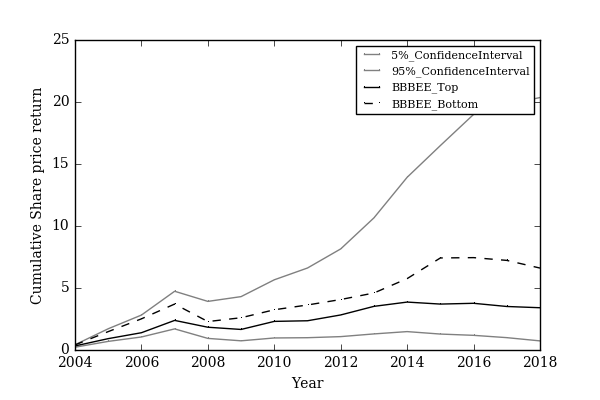
\includegraphics [scale=1]{Images/Bootstrap_All.png} \\
  {\small {\it \caption{Bootstrap entire dataset \label{fig:moun} }}}
\end{figure}
This chart displays four variables the 5\% and 95\% confidence intervals and the share price return of the top and bottom B-BBEE ranking firms. The confidence intervals were generated by bootstrapping the average returns of the entire dataset for each year, and retrieving the 5\% lowest and 5\% highest average returns for this year. These returns, as well as the returns for the top and bottom B-BBEE ranking firms were compounded over time. The top and bottom B-BBEE ranking firms were the average return of top and bottom 30\% ranking firms for each years. This chart shows that the 5\% highest average returns, the 95\% confidence interval rose significantly post 2008, outperforming all other variables handsomely as the average returns compounded aggressively. Similarly, although at a significant smaller compounding rate, the bottom B-BBEE ranking firms rose after 2008. It is particularly striking that from this analysis the bottom ranking B-BBEE firms outperform the top ranking B-BBEE firms. This analysis further shows the the bottom ranking B-BBEE firms do outperform the 5\% low confidence interval. This indicates the relationship between B-BBEE and share price return is insignificant. 

Returning towards a possible bias in the Industrial sector, this study performed the same bootstrap analysis for firms in this sector to answer the sub question: “Did firms operating in a sector with a higher incentive to comply to the B-BBEE policy have higher firm performance?” Below a visualization of the results.
\begin{figure}[!h]
  \centering
  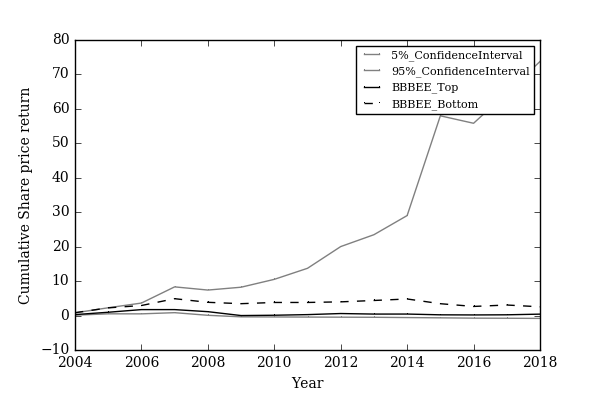
\includegraphics [scale=1]{Images/Bootstrap_Industrials.png} \\
  {\small {\it \caption{Bootstrap Industrials \label{fig:moun} }}}
\end{figure}
This bootstrap did entail a smaller sample size, which might explain that the findings of this chart are an exaggeration of the findings in the bootstrap analysis on the entire dataset. In this dataset, contrary to the idea in the Descriptives section, It appears that the negative relationship between B-BBEE and share price return is close to significant, as the top B-BBEE ranking firms in the Industrial sector remain close to the bottom 5\% confidence interval.

The simulation for Consumer Services also shows a non significant performance of the top ranking B-BBEE firms. \begin{figure}[!h]
  \centering
  \includegraphics [scale=1]{"Images/Bootstrap_Consumer Services_Cumulative"} \\
  {\small {\it \caption{Bootstrap Consumer Services \label{fig:moun} }}}
\end{figure}
This sector however does display that the top ranking B-BBEE firms outperformed the bottom ranking B-BBEE firms. Recall, from the section “B-BBEE and signalling effects” that theory states that  consumer behavior could express their values regarding empowerment in their consumption pattern [34, p378]. This chart shows weak evidence of this statement.

The other sector bootstrap simulation can be found in Appendix C. Note however, that the sectors Telecommunications, Technology, Health Care and Consumer Goods consisted of less than 8 observations in each year. This could affect the robustness of the findings per sector. 
\section{Summary and conclusion}
Descriptive statistics were used to inform the reader about the general characteristics of the dataset used to test the hypothesis. These displayed a sizeable sample size, with at most 816 observations. Furthermore, the sample size did display a positive bias towards the Industrial sector and a negative bias towards the Financial sector, which could be attributed to the sector’s incentive to comply to B-BBEE. Although the dataset did present outliers, the outliers did not meaningfully alter the conclusions on the regression analyses used to answer the research sub question: “What was the long term relationship between Broad-Based Black Economic Empowerment policy on firm profitability of the Johannesburg Stock Exchange-listed companies over the period 2004 - 2018?”. Both outlier and non outlier adjusted regressions of Model 1, the FF model, indicate that the relationship between B-BBEE rank and two, three and four years share price return  was significantly negative. Model 2, the MF model, confirmed the finding on three and four years share price return. The significance levels did differ. For example, the non-outlier adjusted model 1 was significant at 1\% on 3 years share price return, whereas model 2 for this time horizon was significant at 5\%. Further, Model 2, the  MF model, held quite low explanatory value, with r squared below 5\%, whereas model 1, the FF model generated acceptable r squared equal to or larger than 14\%. 

Regressions were tested on sub sections of the dataset to answer the research sub question: “What was the long term relationship between B-BBEE policy and firm performance among the three B-BBEE policy periods?”. These regressions did not display materially different findings from the tests on the entire time period. The period 2013-2018 did display more pronounced significant negative relationship between B-BBEE and two, three and four years share price return compared to the entire dataset. Compared to the entire dataset, the period 2007-2013 showed  a less negative relationship, albeit insignificant, between B-BBEE and share price returns on two, three and four years basis. The period 2004 - 2007 showed a insignificant positive relationship between B-BBEE and two years share price return.

Finally, the bootstrap method was used to investigate whether the research sub question “What was the long term relationship between Broad-Based Black Economic Empowerment policy on firm profitability of the Johannesburg Stock Exchange-listed companies over the period 2004 - 2018?” differed from the findings using the regression models. The bootstrap method showed that the compounded one year share price returns of the Top B-BBEE ranking firms fell in the 95\% and 5\% confidence interval, thus showing no significant relationship. It was found that the bottom B-BBEE ranking firms outperformed the top B-BBEE ranking firms, further adding to the notion that the relationship between B-BBEE and share price return could be negative. Finally, the Bootstrap method found that in the Industrial sector, a sector with an incentive to comply to B-BBEE, the share price return of top ranking B-BBEE firms moved closely to the bottom 5\% confidence interval. Regarding sub question: “Did firms operating in a sector with a higher incentive to comply to the B-BBEE policy have higher firm performance?”, the Bootstrap method for Industrial indicated that these firms did not have higher firm performance.

Returning to the hypothesis in the methodology, the finding in the empirical analysis indicate a negative relationship between B-BBEE policy and firm performance. Therefore the null hypothesis "There relationship between B-BBEE aggregate score and share price return of Johannesburg Stock Exchange-listed companies is positive", is rejected.